\documentclass[a4paper,10pt]{article}
\usepackage[top=3cm, bottom=3cm, left=3cm, right=3cm]{geometry}
\usepackage[T1]{fontenc}
\usepackage[utf8]{inputenc}
\usepackage{lmodern}
\usepackage[francais]{babel}
\usepackage{graphicx}
\usepackage{caption}
\usepackage{subcaption}
\usepackage{eurosym}
\usepackage{hyperref}
\usepackage{csvsimple}
\usepackage{array}
\usepackage{longtable}
\usepackage{placeins}

\begin{document}

\begin{titlepage}
  \newcommand{\HRule}{\rule{\linewidth}{0.5mm}} % Defines a new command for the horizontal lines, change thickness here

  \center % Center everything on the page
   
  %----------------------------------------------------------------------------------------
  %	HEADING SECTIONS
  %----------------------------------------------------------------------------------------

  \textsc{\LARGE INSA de Lyon}\\[1.5cm] % Name of your university/college
  \textsc{\Large PLD-Agile}\\[0.5cm] % Major heading such as course name
  %\textsc{\large Compte rendue de TP}\\[0.5cm] % Minor heading such as course title

  %----------------------------------------------------------------------------------------
  %	TITLE SECTION
  %----------------------------------------------------------------------------------------

  \HRule \\[0.4cm]
  { \huge \bfseries Compte rendu de dernière itération}\\[0.4cm] % Title of your document
  \HRule \\[1.5cm]
   
  %----------------------------------------------------------------------------------------
  %	AUTHOR SECTION
  %----------------------------------------------------------------------------------------

  % If you don't want a supervisor, uncomment the two lines below and remove the section above
  \Large \emph{Auteurs:}\\[1cm]
  \begin{table}[h]
    \begin{center}
      \begin{tabular}{r l}
         Sebastien & \textsc{Di Giovanni} \\
         Hugo & \textsc{Moynac} \\
         Ruben & \textsc{Pericas Moya} \\
         François & \textsc{Robion} \\
         Charles & \textsc{Samborski} \\
         Nicolas & \textsc{Six} \\[3cm]
      \end{tabular}
    \end{center}
  \end{table}
  
  %----------------------------------------------------------------------------------------
  %	DATE SECTION
  %----------------------------------------------------------------------------------------

  {\large \today}\\[3cm] % Date, change the \today to a set date if you want to be precise

  %----------------------------------------------------------------------------------------
  %	LOGO SECTION
  %----------------------------------------------------------------------------------------

  %\includegraphics{Logo}\\[1cm] % Include a department/university logo - this will require the graphicx package
   
  %----------------------------------------------------------------------------------------

  \vfill % Fill the rest of the page with whitespace

\end{titlepage}
\tableofcontents
\pagebreak

\listoffigures
\pagebreak


\section{Retour sur le PLD Agile}
\subsection{Organisation des séances}
\paragraph{}
Nous avons trouvé dommages que les séances s’enchaînent à deux par semaines, car cela nous laisser peu de temps pour travailler entre chaque séance. De plus, le PLD Mars était effectué sur la même période de temps, les deux PLD combiné représentait une charge de travail importante. 

\subsection{Présentation du sujet}
\paragraph{}
Le sujet était intéressant dans le fait qu’il était très complet. En effet, les projets de 3IF ne traitaient la plupart du temps que d’un seul point (algorithmie, IHM, stockage de données…), alors que le PLD, en traitant de tous ces points, permettait d’aborder chacun de ces problèmes, mais aussi les difficultés qu’ils pouvaient y avoir à relier ces parties.

\subsection{Organisation de l’agilité}
\paragraph{}
J’ai eu l’impression que l’organisation au sein de l’équipe se faisait en très grande partie lors des séances. C’est-à-dire qu’on avançait chacun de son côté chez nous, et le cours nous servait de recentrage. 

\FloatBarrier
\section{Description textuelle des cas d’utilisation}
  \input{project/use-cases/add-delivery-address-in-delivery-request_fr_FR.tex}
  \input{project/use-cases/remove-delivery-address-in-delivery-request_fr_FR.tex}
  \input{project/use-cases/undo-modification-on-delivery-request_fr_FR.tex} 
  \input{project/use-cases/redo-modification-on-delivery-request_fr_FR.tex} 
  \input{project/use-cases/generate-itinerary-text_fr_FR.tex} 

  
%mettre à jour avec les donnée rétro générer  
\FloatBarrier
%generated tex file
\begin{figure}[h!]
    		\begin{center}
      			\includegraphics[width=0.3\linewidth,height=.7\paperheight,keepaspectratio]{retrogenerated_uml/exceptionwindow.png}
      			\caption{Diagramme de classe du package exceptionwindow}
    		\end{center}
  	\end{figure}
\begin{figure}[h!]
    		\begin{center}
      			\includegraphics[width=\linewidth,height=.7\paperheight,keepaspectratio]{retrogenerated_uml/citymapdetails.png}
      			\caption{Diagramme de classe du package citymapdetails}
    		\end{center}
  	\end{figure}
\begin{figure}[h!]
    		\begin{center}
      			\includegraphics[width=0.3\linewidth,height=.7\paperheight,keepaspectratio]{retrogenerated_uml/intersectioncard.png}
      			\caption{Diagramme de classe du package intersectioncard}
    		\end{center}
  	\end{figure}
\begin{figure}[h!]
    		\begin{center}
      			\includegraphics[width=0.3\linewidth,height=.7\paperheight,keepaspectratio]{retrogenerated_uml/informationarea.png}
      			\caption{Diagramme de classe du package informationarea}
    		\end{center}
  	\end{figure}
\begin{figure}[h!]
    		\begin{center}
      			\includegraphics[width=\linewidth,height=.7\paperheight,keepaspectratio]{retrogenerated_uml/mapscreen.png}
      			\caption{Diagramme de classe du package mapscreen}
    		\end{center}
  	\end{figure}
\begin{figure}[h!]
    		\begin{center}
      			\includegraphics[width=\linewidth,height=.7\paperheight,keepaspectratio]{retrogenerated_uml/components.png}
      			\caption{Diagramme de classe du package components}
    		\end{center}
  	\end{figure}
\begin{figure}[h!]
    		\begin{center}
      			\includegraphics[width=\linewidth,height=.7\paperheight,keepaspectratio]{retrogenerated_uml/events.png}
      			\caption{Diagramme de classe du package events}
    		\end{center}
  	\end{figure}
\begin{figure}[h!]
    		\begin{center}
      			\includegraphics[width=\linewidth,height=.7\paperheight,keepaspectratio]{retrogenerated_uml/timefield.png}
      			\caption{Diagramme de classe du package timefield}
    		\end{center}
  	\end{figure}
\begin{figure}[h!]
    		\begin{center}
      			\includegraphics[width=0.3\linewidth,height=.7\paperheight,keepaspectratio]{retrogenerated_uml/deliveryrequestdetails.png}
      			\caption{Diagramme de classe du package deliveryrequestdetails}
    		\end{center}
  	\end{figure}
\begin{figure}[h!]
    		\begin{center}
      			\includegraphics[width=\linewidth,height=.7\paperheight,keepaspectratio]{retrogenerated_uml/application.png}
      			\caption{Diagramme de classe du package application}
    		\end{center}
  	\end{figure}
\begin{figure}[h!]
    		\begin{center}
      			\includegraphics[width=\linewidth,height=.7\paperheight,keepaspectratio]{retrogenerated_uml/waypointcard.png}
      			\caption{Diagramme de classe du package waypointcard}
    		\end{center}
  	\end{figure}
\begin{figure}[h!]
    		\begin{center}
      			\includegraphics[width=\linewidth,height=.7\paperheight,keepaspectratio]{retrogenerated_uml/planningdetails.png}
      			\caption{Diagramme de classe du package planningdetails}
    		\end{center}
  	\end{figure}
\begin{figure}[h!]
    		\begin{center}
      			\includegraphics[width=\linewidth,height=.7\paperheight,keepaspectratio]{retrogenerated_uml/mapcanvas.png}
      			\caption{Diagramme de classe du package mapcanvas}
    		\end{center}
  	\end{figure}
\begin{figure}[h!]
    		\begin{center}
      			\includegraphics[width=0.3\linewidth,height=.7\paperheight,keepaspectratio]{retrogenerated_uml/main.png}
      			\caption{Diagramme de classe du package main}
    		\end{center}
  	\end{figure}
\begin{figure}[h!]
    		\begin{center}
      			\includegraphics[width=\linewidth,height=.7\paperheight,keepaspectratio]{retrogenerated_uml/tsp.png}
      			\caption{Diagramme de classe du package tsp}
    		\end{center}
  	\end{figure}
\begin{figure}[h!]
    		\begin{center}
      			\includegraphics[width=\linewidth,height=.7\paperheight,keepaspectratio]{retrogenerated_uml/command.png}
      			\caption{Diagramme de classe du package command}
    		\end{center}
  	\end{figure}
\begin{figure}[h!]
    		\begin{center}
      			\includegraphics[width=\linewidth,height=.7\paperheight,keepaspectratio]{retrogenerated_uml/map.png}
      			\caption{Diagramme de classe du package map}
    		\end{center}
  	\end{figure}
\begin{figure}[h!]
    		\begin{center}
      			\includegraphics[width=\linewidth,height=.7\paperheight,keepaspectratio]{retrogenerated_uml/xml.png}
      			\caption{Diagramme de classe du package xml}
    		\end{center}
  	\end{figure}
\begin{figure}[h!]
    		\begin{center}
      			\includegraphics[width=\linewidth,height=.7\paperheight,keepaspectratio]{retrogenerated_uml/exception.png}
      			\caption{Diagramme de classe du package exception}
    		\end{center}
  	\end{figure}
\begin{figure}[h!]
    		\begin{center}
      			\includegraphics[width=0.3\linewidth,height=.7\paperheight,keepaspectratio]{retrogenerated_uml/tools.png}
      			\caption{Diagramme de classe du package tools}
    		\end{center}
  	\end{figure}
\begin{figure}[h!]
    		\begin{center}
      			\includegraphics[width=0.3\linewidth,height=.7\paperheight,keepaspectratio]{retrogenerated_uml/pdf.png}
      			\caption{Diagramme de classe du package pdf}
    		\end{center}
  	\end{figure}
\begin{figure}[h!]
    		\begin{center}
      			\includegraphics[width=\linewidth,height=.7\paperheight,keepaspectratio]{retrogenerated_uml/services.png}
      			\caption{Diagramme de classe du package services}
    		\end{center}
  	\end{figure}
\begin{figure}[h!]
    		\begin{center}
      			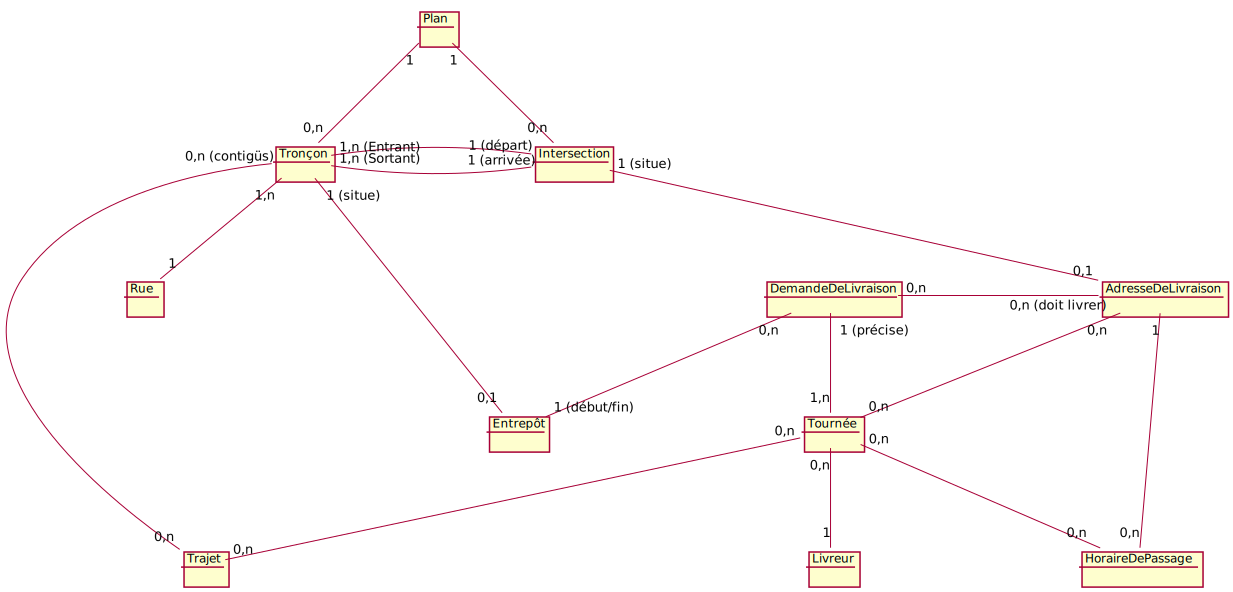
\includegraphics[width=\linewidth,height=.7\paperheight,keepaspectratio]{retrogenerated_uml/model.png}
      			\caption{Diagramme de classe du package model}
    		\end{center}
  	\end{figure}
\begin{figure}[h!]
    		\begin{center}
      			\includegraphics[width=\linewidth,height=.7\paperheight,keepaspectratio]{retrogenerated_uml/java.png}
      			\caption{Diagramme de classe du package java}
    		\end{center}
  	\end{figure}


\FloatBarrier
\input{docs/architecture.tex}


\FloatBarrier
\section{Couverture de tests}
\subsection{Réalisation des tests}
\paragraph{}
Nous avons utilisé Junit pour les tests unitaires afin de vérifier le bon fonctionnement du parser, de l’algorithme de Dijkstra ainsi que de l’algorithme du TSP.

\subsection{Tests de non régression}
\paragraph{}
L’intégration de Travis Cl sur Slack que nous utilisons comme outil de communication nous a permis d’observer les résultats de l’ensemble des tests unitaires à chaque push sur le répertoire git et ainsi de contrôler la non régression du code.

\subsection{Couverture de code}
\paragraph{}
La couverture de code réalise avec EclEmma indique un résultat de 43 \%. Cela s’explique par la part importante de code lié à l’IHM qui, elle, n’a pas été testé. 

\begin{figure}[h!]
  \begin{center}
    \includegraphics[width=\linewidth,height=.7\paperheight,keepaspectratio]{couverture.png}
    \caption{Couverture des tests}
    \label{fig:}
  \end{center}
\end{figure}



%mettre à jour les planning des différentes itérations
\FloatBarrier
\section{Planning effectif de la première itération}
  \input{charges/charges_it1.tex}
  
\FloatBarrier
\section{Planning effectif de la deuxième itération}
  \input{charges/charges_it2.tex}
  
\FloatBarrier
\section{Planning effectif de la troisième itération}
  \input{charges/charges_it3.tex}

\end{document}
